%<dscrpt>Introduction à l'algorithmique</dscrpt>
% <rel_id_elt_parent>6469</rel_id_elt_parent> id de ``Algorithmique''
% <rel_id_type_rel>14</rel_id_type_rel> id de ``contient sana ordre l'élément''
%!  pour pdfLatex
\documentclass[a4paper]{article}
%\usepackage[hmargin={1.5cm,1.5cm},vmargin={2.4cm,2.4cm},headheight=13.1pt]{geometry}
\usepackage[a4paper,landscape,twocolumn,
            hmargin=1.8cm,vmargin=2.2cm,headheight=13.1pt]{geometry}

\usepackage[pdftex]{graphicx,color}
\usepackage[pdftex,colorlinks={true},urlcolor={blue},pdfauthor={remy Nicolai}]{hyperref}

\usepackage[T1]{fontenc}
\usepackage[utf8]{inputenc}

\usepackage{lmodern}
\usepackage[frenchb]{babel}

\usepackage{fancyhdr}
\pagestyle{fancy}

\usepackage{floatflt}
\usepackage{maths}

\usepackage{parcolumns}
\setlength{\parindent}{0pt}

\usepackage{caption}
\usepackage{subcaption}

\usepackage{makeidx}

\usepackage[french,ruled,vlined]{algorithm2e}
\SetKwComment{Comment}{\#}{}
\SetKwFor{Tq}{tant que}{}{}
\SetKwFor{Pour}{pour}{}{}
\DontPrintSemicolon
\SetAlgoLined

\usepackage{listings}
\lstset{language=Python,frame=single}
\lstset{literate=
  {á}{{\'a}}1 {é}{{\'e}}1 {í}{{\'i}}1 {ó}{{\'o}}1 {ú}{{\'u}}1
  {Á}{{\'A}}1 {É}{{\'E}}1 {Í}{{\'I}}1 {Ó}{{\'O}}1 {Ú}{{\'U}}1
  {à}{{\`a}}1 {è}{{\`e}}1 {ì}{{\`i}}1 {ò}{{\`o}}1 {ù}{{\`u}}1
  {À}{{\`A}}1 {È}{{\'E}}1 {Ì}{{\`I}}1 {Ò}{{\`O}}1 {Ù}{{\`U}}1
  {ä}{{\"a}}1 {ë}{{\"e}}1 {ï}{{\"i}}1 {ö}{{\"o}}1 {ü}{{\"u}}1
  {Ä}{{\"A}}1 {Ë}{{\"E}}1 {Ï}{{\"I}}1 {Ö}{{\"O}}1 {Ü}{{\"U}}1
  {â}{{\^a}}1 {ê}{{\^e}}1 {î}{{\^i}}1 {ô}{{\^o}}1 {û}{{\^u}}1
  {Â}{{\^A}}1 {Ê}{{\^E}}1 {Î}{{\^I}}1 {Ô}{{\^O}}1 {Û}{{\^U}}1
  {œ}{{\oe}}1 {Œ}{{\OE}}1 {æ}{{\ae}}1 {Æ}{{\AE}}1 {ß}{{\ss}}1
  {ű}{{\H{u}}}1 {Ű}{{\H{U}}}1 {ő}{{\H{o}}}1 {Ő}{{\H{O}}}1
  {ç}{{\c c}}1 {Ç}{{\c C}}1 {ø}{{\o}}1 {å}{{\r a}}1 {Å}{{\r A}}1
  {€}{{\euro}}1 {£}{{\pounds}}1 {«}{{\guillemotleft}}1
  {»}{{\guillemotright}}1 {ñ}{{\~n}}1 {Ñ}{{\~N}}1 {¿}{{?`}}1
}

%pr{\'e}sentation des compteurs de section, ...
\makeatletter
\renewcommand{\thesection}{\Roman{section}.}
\renewcommand{\thesubsection}{\arabic{subsection}.}
\renewcommand{\thesubsubsection}{\arabic{subsubsection}.}
\renewcommand{\labelenumii}{\theenumii.}
\makeatother


\newtheorem*{thm}{Théorème}
\newtheorem{thmn}{Théorème}
\newtheorem*{prop}{Proposition}
\newtheorem{propn}{Proposition}
\newtheorem*{pa}{Présentation axiomatique}
\newtheorem*{propdef}{Proposition - Définition}
\newtheorem*{lem}{Lemme}
\newtheorem{lemn}{Lemme}

\theoremstyle{definition}
\newtheorem*{defi}{Définition}
\newtheorem*{nota}{Notation}
\newtheorem*{exple}{Exemple}
\newtheorem*{exples}{Exemples}


\newenvironment{demo}{\renewcommand{\proofname}{Preuve}\begin{proof}}{\end{proof}}
%\renewcommand{\proofname}{Preuve} doit etre après le begin{document} pour fonctionner

\theoremstyle{remark}
\newtheorem*{rem}{Remarque}
\newtheorem*{rems}{Remarques}

%\usepackage{maths}
%\newcommand{\dbf}{\leftrightarrows}

%En tete et pied de page
\lhead{Informatique}
%\chead{Introduction aux systèmes informatiques}
\rhead{MPSI B Hoche}
\lfoot{\tiny{Cette création est mise à disposition selon le Contrat\\ Paternité-Partage des Conditions Initiales à l'Identique 2.0 France\\ disponible en ligne http://creativecommons.org/licenses/by-sa/2.0/fr/  
} 
\rfoot{\tiny{Rémy Nicolai \jobname \; \today } }
}
\makeindex


%En tete et pied de page
\lhead{Cours IPT}
\chead{Introduction à l'algorithmique}

\begin{document}
On ne cherchera pas à définir ce qu'est un algorithme\index{algorithme}, on se contentera de l'image d'une \emph{recette de cuisine abstraite}.

La première partie de ce document présente sur un exemple imagé des notions importantes pour implémenter un algorithme dans un langage de programation. La seconde présente un algorithme particulier qui joue un rôle fondamental dans la manière de gérer des objets de type "entier".

\section{La cuisson des coquillettes}
Partons de la description de l'algorithme dans un livre de cuisine (figure \ref{fig:introalgo_1}) qui date des années 1960. 
\begin{figure}[ht]
 \centering
 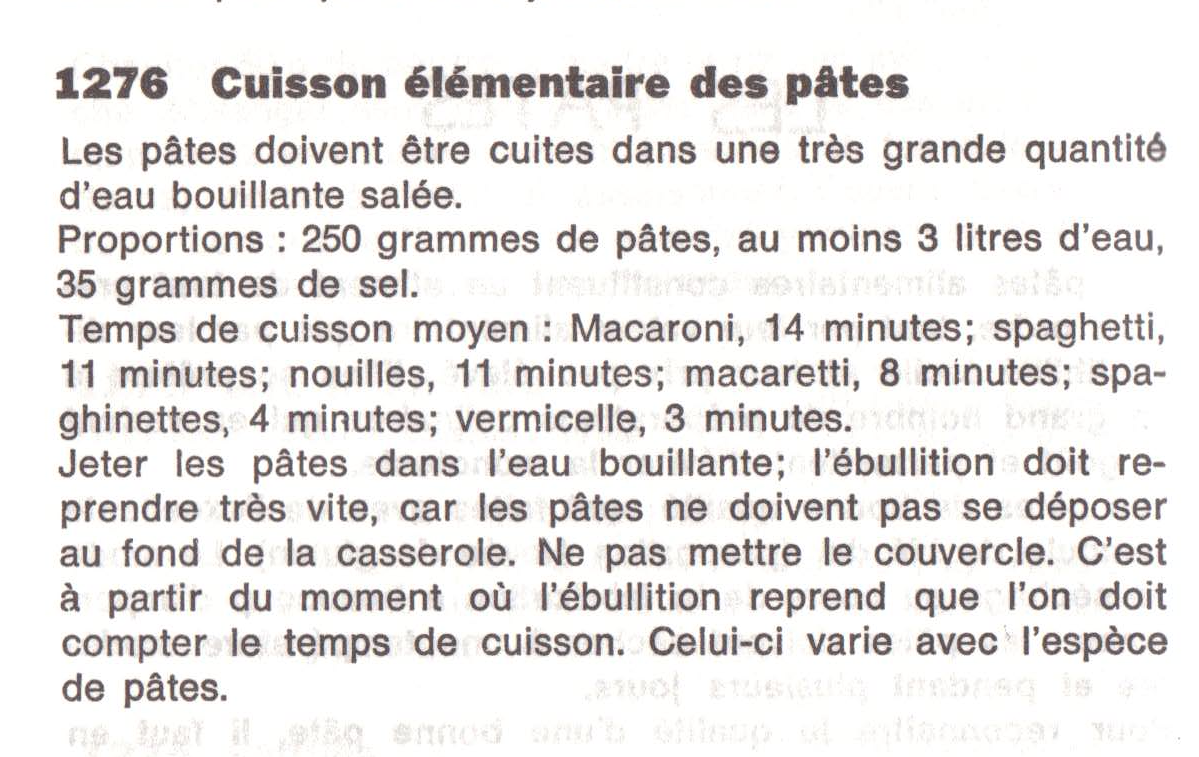
\includegraphics[width=7cm]{introalgo_1.png}
 \caption{Un algorithme en langage "naturel" (Ginette Mathiot)}
 \label{fig:introalgo_1}
\end{figure}
On se propose de traduire (\emph{implémenter}) l'algorithme de cuisson des pâtes en utilisant des conventions plus modernes et qui se prêtent mieux à la généralisation.

On peut simplement aller à la ligne entre chaque commande
\begin{verbatim}
utiliser : 250 g de pâtes, 35 g de sel, 3 litres d'eau
 -faire bouillir de l'eau salée
 -mettre les pâtes dans l'eau
 -laisser cuire 5mn
\end{verbatim} 
Chacune des trois commandes précédentes est un enchaînement de commandes plus élémentaires que l'on peut choisir de préciser. On le fait pour introduire des concepts de base en programmation.
\begin{description}
 \item[nom] \index{nom} \index{variable} Certains langages ont des variables, Python ne connait que des noms ce qui n'est pas la même chose. Un nom référence un objet.
 \item[objet] Une donnée que le langage sait stocker et manipuler.\index{objet} Il existe plusieurs types d'objets, certains types peuvent être modifiables (mutable) d'autres non. \emph{Littéral}\index{littéral} (literals).
 \item[expression] \index{expression}Une phrase formée avec des littéraux, des noms, des \emph{opérateurs} des parenthèses.
 \item[référence] (assignation, "="). \index{assignation}Le mot à gauche de "=" devient un nom pour l'objet représenté par ce qui est à droite (nom ou expression)
 \item[fonction] Une fonction "fait quelque chose"\index{fonction} avec les \emph{paramètres}\index{fonction!paramètres} qui lui sont passés et \emph{renvoie}\index{fonction!renvoi} ou non un objet. Chaque fonction n'accepte que des paramètres désignant des objets de types particuliers définis à la construction de la fonction. Certaines fonctions sont attachées à des certains objets, on les appelle alors des \emph{méthodes} \index{objet:méthodes} de ce type d'objet.
\end{description}

\bigskip
\begin{parcolumns}[rulebetween,distance=1cm]{2}
 \colchunk{Cassy $\leftarrow$ une casserole\newline Eg $\leftarrow$ un égouttoir}
 \colchunk{des assignations (références) Cassy est le nom d'un objet de type "casserole", Eg est le nom d'un objet de type "égouttoir".}
 \colplacechunks
  
 \colchunk{Cassy.ajouter(eau + sel)}
 \colchunk{eau + sel est une expression. Les casseroles comme les égouttoirs sont des "récipients" un récipient possède les méthodes "ajouter()" et "vider()"}
 \colplacechunks
  
 \colchunk{faireBouillir(Cassy)}
 \colchunk{"faireBouillir" est une fonction qui ne renvoie rien mais modifie l'objet qui lui est passé. }
 \colplacechunks
  
 \colchunk{Cassy.ajouter(pâtes)}
 \colchunk{la méthode "ajouter" modifie l'objet auquel elle est attachée.}
 \colplacechunks
  
 \colchunk{chauffer(Cassy,5)}
 \colchunk{une fonction avec deux paramètres très différents.}
 \colplacechunks
  
 \colchunk{Eg.ajouter(Cassy.vider())}
 \colchunk{la méthode "vider" renvoie un objet}
 \colplacechunks
 
 \colchunk{Eg.secouer()}
 \colchunk{}
 \colplacechunks

 \colchunk{Cassy.ajouter(Eg.vider() + beurre)}
 \colchunk{}
 \colplacechunks

 \colchunk{Eg.oublier()}
 \colchunk{ceci est inutile pour les langages modernes}
 \colplacechunks

\end{parcolumns}

Introduisons  la notion de \emph{structure de contrôle}\index{structure de contrôle} dans l'enchaînement des commandes. Une structure de contrôle contient des \emph{conditions}\index{condition} (Une condition est une expression qui s'évalue à une valeur booléenne) et des \emph{blocs d'instruction}\index{bloc d'instruction}. On va évaluer quelque chose (une condition) à "vrai" ou "faux" et diriger vers des enchaînements différents (blocs) suivant le résultat. Il existe essentiellement deux structures de contrôle
\begin{itemize}
  \item \emph{branchement} \texttt{if} \index{structure de contrôle! branchement \texttt{if}}
  \item \emph{boucle} \texttt{while} \index{structure de contrôle! boucle \texttt{while}}
\end{itemize}

Pour préciser \verb|faireBouillir| donnons les fonctions plus élémentaires qu'elle va utiliser:
\begin{itemize}
 \item \verb|bonAchauffer(r)|.  \verb|r| est le nom d'un récipient. L'appel renvoie l'objet de type booléen \verb|VRAI| ou \verb|FAUX| suivant ce que désigne \verb|r| (il contient de l'eau et il n'est pas en plastique). L'état du récipient n'est pas modifié par l'appel.
 \item \verb|chauffer(r,t)|.  \verb|r| est le nom d'un récipient, \verb|t| est le nom d'une durée en minutes.  L'appel ne renvoie rien mais modifie l'état du récipient (de son contenu).
 \item \verb|tempInt(r)|. Renvoie la température du liquide contenu dans le récipient.
\end{itemize}
On peut alors détailler la fonction elle même
\begin{verbatim}
faireBouillir est une fonction de paramètre r
   si non bonAchauffer(r):
       terminer en renvoyant un message d'erreur
   tant que tempInt(r)< 100
       chauffer(r,1)
\end{verbatim}
Attention, rien n'assure que cette boucle se termine, on parle alors de \emph{boucle infinie}.\index{boucle infinie} Il convient d'ajouter une structure de sécurité.
La syntaxe Python de ces structures de contrôle sera vue en TP.

\section{Numération dans une base.}
\begin{prop}
 Soit $b$ un entier naturel supérieur ou égal à $2$. Pour tout entier naturel $x$ entre $0$ et $b^n-1$, il existe un unique $n$-uplet
\begin{displaymath}
 (a_0,a_1,\cdots,a_{n-1})\in \{0,1,\cdots,b-1\}^n
\end{displaymath}
tel que 
\begin{displaymath}
 x = a_0 + a_1 b +\cdots +a_{n-1}b^{n-1}
\end{displaymath}
\end{prop}
Cette proposition traduit l'existence et l'unicité de la décomposition d'un entier dans une base arbitraire. On utilise en particulier les bases $b=2$ (binaire), $b=10$ (décimale), $b=16$ (héxadécimal), $b=20$ \footnote{voir le système de numération maya. Cette base semble aussi avoir été utilisée par les Gaulois, le 80 quatre-vingt en serait un lointain vestige (ref wikipédia) }, $b=60$ (sexagésimale) \footnote{utilisé par les mésopotamiens voir en particulier les tablettes cuneiformes de Plimpton}
\begin{demo}
 Pour démontrer cette proposition, on va remarquer qu'elle est équivalente à la bijectivité d'une certaine application entre deux ensembles finis ayant le même nombre d'éléments. Pour une telle application, l'injectivité entraîne la surjectivité donc la bijectivité.\newline
La démonstration de l'injectivité est \emph{constructive}. Si un entier est décomposé alors chaque $a_i$ se calcule algorithmiquement en fonction de $x$ et de $b$. Ceci assure l'unicité de la décomposition donc l'injectivité de la fonction.

Considérons la fonction
\begin{displaymath}
 \Phi\left\lbrace 
\begin{aligned}
\{0,1,\cdots,b-1\}^n \rightarrow& \{0,1,\cdots,b^n-1\}\\
(a_0,a_1,\cdots,a_{n-1}) \rightarrow& a_0 + a_1 b +\cdots +a_{n-1}b^{n-1} 
\end{aligned}
\right.
\end{displaymath}
En fait, il faut commencer par montrer que
\begin{displaymath}
 a_0 + a_1 b +\cdots +a_{n-1}b^{n-1}\in \{0,1,\cdots,b^n-1\}
\end{displaymath}
Ceci résulte de l'encadrement
\begin{multline*}
 0\leq a_0 + a_1 b +\cdots +a_{n-1}b^{n-1} 
\leq (b-1) + (b-1) b +\cdots +(b-1)b^{n-1}\\
\leq (b-1)(1+b+\cdots +b^{n-1})=b^n-1
\end{multline*}
On démontre exactement de la même manière que, pour des $m\leq n$:
\begin{displaymath}
 a_0 + a_1 b +\cdots +a_{m-1}b^{m-1}\in \{0,1,\cdots,b^m-1\}
\end{displaymath}
Ceci servira plus loin pour justifier un des deux algorithmes proposés.\newline
La proposition est exactement équivalente à la bijectivité de la fonction $\Phi$. Les ensembles de départ et d'arrivée ont le même nombre d'éléments à savoir $b^n$.\newline
Si la fonction $\Phi$ est injective, les images sont deux à deux distinctes. Il y a donc autant d'images distinctes que d'éléments dans l'ensemble de départ. Mais alors tous les $b^n$ éléments de l'ensemble d'arrivée sont des images puisque cet ensemble ne contient que $b^n$ éléments.\newline
Démontrons maintenant l'injectivité\footnote{On peut présenter cette démonstration comme une analyse-synthèse. L'analyse correspond à l'injectivité ou à l'unicité, son argumentation est algorithmique. La synthèse correspond à la surjectivité ou à l'existence, son argumentation repose sur la théorie des ensembles}. On suppose
\begin{displaymath}
 x=a_0 + a_1 b +\cdots +a_{n-1}b^{n-1}
\end{displaymath}
On peut adopter un algorithme "glouton" en cherchant d'abord les "plus gros morceaux" c'est à dire le nombre $a_{n-1}$ de $b^{n-1}$ contenus dans $x$. Comme 
\begin{displaymath}
 0\leq a_0 + a_1 b +\cdots +a_{n-2}b^{n-2}\leq b^{n-1}-1
\end{displaymath}
ce nombre est le reste de la division de $x$ par $b^{n-1}$ et $a_{n-1}$ en est le quotient. Ceci assure l'unicité de $a_{n-1}$ et on peut poursuivre le raisonnement en divisant le reste précédent par $b^{n-2}$.\newline
On peut aussi procéder en partant du bas. Dans la division par $b$ de
\begin{align*}
 x= a_0 + a_1 b +\cdots +a_{m-1}b^{m-1} = a_0 +(a_1+a_2b+\cdots+a_{n-1}b^{n-2})b
\end{align*}
le reste est $a_0$ et le quotient est $a_1+a_2b+\cdots+a_{n-1}b^{n-2}$. Ceci assure l'unicité du $a_0$ et le raisonnement se poursuit en divisant par $b$ le quotient précédent.
\end{demo}
L'expression en pseudo-code de cet algorithme est la suivant
\begin{verbatim}
b <-- la base
x <-- un nombre entier >0
# recherche du plus petit n tel que x<b^n
n <-- 0
p<-- 1
tant que p <= x
  n<-- n+1
  p<-- p*b
#formation du développement
resultat <-- liste vide
p<-- p/b
tant que x>0
  resultat.append(quotient de la div de x par p)
  x<-- reste de la division de x par p
  p<- p/b
print(resultat)
\end{verbatim}
La syntaxe des structures de contrôle sera présentée en détail en TP mais cet exemple (algorithme de numération : les grands d'abord) est une bonne introduction.
\begin{verbatim}
b = 10
x = 259
n = 0
p = 1
#recherche du plus petit n tel que x<b^n
while p <= x:
    n += 1
    p *= b
print(n)
#formation du développement
resultat = []
p = p//b
while x>0:
    resultat.append(x // p)
    x = x % p
    p = p / b
print(resultat) 
\end{verbatim}
On peut aussi implémenter avec les petits d'abords
  \begin{verbatim}
b = 10 ; x = 16**8 ; print(x)
resultat = []
while x > 0 :
    resultat.append(x % b)
    x = x // b
print(resultat)  
\end{verbatim}
Le problème est alors que les décimales sont rangées à l'envers dans la liste. 

\section{Développement d'un réel dans une base}
\subsection{Partie entière et division}
On a déjà vu que tout nombre entier naturel se décompose de manière unique dans une base $b\geq2$ quelconque. Pratiquement, cette décomposition peut se faire en utilisant deux algorithmes: \og les petits d'abord \fg~ ou \og les grands d'abord \fg. On peut étendre ces principes des entiers aux réels.

D'après une propriété de $\R$, tout nombre réel se décompose de manière unique sous la forme
\begin{displaymath}
  \text{un nombre réel} = \text{un nombre entier} + \text{un nombre réel dans $[0,1[$}
\end{displaymath}
Notation
\begin{displaymath}
  x = \underset{\text{partie entière de } x\in \Z }{\underbrace{\lfloor x \rfloor}} + \underset{\in [0,1[ }{\underbrace{\{ x \}}}
\end{displaymath}
On dit aussi que $\{x\}$ est la partie \emph{décimale} de $x$.

Comme $\Q$ est une partie de $\R$, la partie entière rend compte de la division euclidienne arithmétique\newline
Dans la division de $m\in \Z$ par $n\in \N^*$ 
\begin{displaymath}
  m = \underset{\in \Z}{\underbrace{n}}q + \underset{\in \llbracket 0, n\llbracket}{\underbrace{r}}
  \Leftrightarrow \frac{m}{n} = \underset{\in \N}{\underbrace{q}} + \underset{\in [0,1[}{\underbrace{\frac{r}{n}}} 
\end{displaymath}
On en déduit que le quotient de la division de $m$ par $n$ est $\lfloor \frac{m}{n} \rfloor$.
\subsection{Développement pratique d'un réel}
\begin{algorithm}
  $y\longleftarrow \lfloor x \rfloor$\;
  \Tq{ $y > 0$}{
      enregistrer le reste de la division de $y$ par $b$\;
      $y\longleftarrow $ le quotient de la division de $y$ par $b$\;
  }
  \caption{\`A gauche: les petits d'abord.}
  \label{nbbin_1}
\end{algorithm}

\begin{algorithm}
  $y\longleftarrow \{ x \}$\;
  \Tq{ $y > 0$}{
      enregistrer $\lfloor by \rfloor$\;
      $y\longleftarrow \{ by\}$\;
  }
  \caption{\`A droite: les grands d'abord.}
  \label{nbbin_2}
\end{algorithm}
Soit $b$ une base fixée (entier naturel strictement plus grand que $1$, le développement d'un nombre réel strictement positif $x$  s'effectue de la manière suivante :
\begin{itemize}
  \item $x = \lfloor x \rfloor + \{x\}$
  \item à gauche : \og les petits d'abord \fg appliqué = $\lfloor x \rfloor$.
  \item à droite : \og les grands d'abord \fg appliqué = $\{ x \}$.
\end{itemize}

Dans l'algorithme \ref{nbbin_1}, on peut remarquer que, à chaque itération, le nombre entier naturel désigné par $y$ diminue strictement ce qui assure que la boucle se termine. En revanche dans l'algorithme \ref{nbbin_2}, $y$ désigne un nombre réel dans $[0,1[$ dont on ne sait pas grand-chose. Rien ne permet d'affirmer qu'il devienne nul et que l'on sorte de la boucle. 

Le développement en base $b$ d'un nombre réel $x>0$ conduit donc à une suite $\left( a_n\right)_{n\leq m_x}$ d'éléments de $\llbracket 0 , b \llbracket$ où $m_x$ est un entier relatif. Les coefficients d'indices positifs correspondent au développement de la partie entière.


Exemple: développement de $7.3$ en base $2$. on trouve $111.01001\,1001\,1001\,\cdots$.

\subsection{Questions mathématiques}
La partie gauche du développement précédent correspond au développement en base $b$ de la partie entière.

En adoptant une notation séquentielle, le développement pratique (partie droite) détaillé plus haut s'écrit
\begin{displaymath}
\left. 
\begin{aligned}
  a_{n+1} &= \lfloor by_n\rfloor \\ y_{n+1} &= \{ny_n\}
\end{aligned}
\right\rbrace
\Rightarrow by_n = a_{n+1} + y_{n+1}
\Rightarrow y_n = \frac{a_{n+1}}{b} + \frac{a_{n+1}}{b}
\end{displaymath}
Cela montre qu'il existe des nombres 
\begin{displaymath}
a_1, a_2, \cdots, a_n \in \llbracket 0, b\llbracket, \hspace{0.5cm} y_n \in [0,1[  
\end{displaymath}
tels que 
\begin{displaymath}
  x = \lfloor x \rfloor + a_1b^{-1} + a_2b^{-2} + \cdots + + a_nb^{-n} + y_nb^{-n}  
\end{displaymath}
Ce formalisme permet de poser des questions:
\begin{itemize}
  \item l'algorithme de la partie droite se termine-t-il?
  \item dans le cas où il ne se termine pas, la suite 
\begin{displaymath}
  \left( a_1b^{-1} + a_2b^{-2} + \cdots + + a_nb^{-n}\right)_{n\in \N^*}
\end{displaymath}
converge-t-elle ? vers $\{x\}$?
\end{itemize}
Pour un $x$ donné, l'algorithme se termine si et seulement si il existe un entier $n$ tel que $xb^n \in \Z$. Pour chaque base $b$, on définit un ensemble particulier formé par les nombres $x$ vérifiant cette propriété. On peut remarquer que tous ces nombres sont rationnels mais que tous les rationnels ne sont pas de cette forme. Lorsque $b=10$ cet ensemble est noté $\D$ (ensemble des nombres décimaux). Lorsque $b=2$, cet ensemble est noté $\B$ (ensemble des nombres binaires).
\begin{align*}
  &\text{nombres binaires}:& &x\in \B \Leftrightarrow \exists n \in\N \text{ tel que } x\,2^{n} \in \Z \\
  &\text{nombres décimaux}:& &x\in \D \Leftrightarrow \exists n \in\N \text{ tel que } x\,10^{n} \in \Z 
\end{align*}
Un nombre décimal est-il binaire? Non! Un nombre binaire est-il décimal? Oui!
Lorsque l'algorithme ne se termine pas, la suite converge vers $\{x\}$ car 
\begin{equation}
  \{x\} - \left( a_1b^{-1} + a_2b^{-2} + \cdots +  a_nb^{-n}\right)  = \frac{y_n}{b^n} \text{ avec } 0 < y_n < b \label{reste}
\end{equation}

Si un $y_n = 0$, on choisit de poser $a_{n+1} = a_{n+2} = \cdots = 0$ de manière à former une suite de $a_k$ dans tous les cas. Cette suite est le développement en base $b$ de $\{x\}$.

Pour chaque nombre réel dans $[0,1[$
\begin{itemize}
  \item L'algorithme associe une unique suite $\left( a_n\right)_{n\in \N}$ d'éléments de $\llbracket 0, b\llbracket$ appelé développement en base $b$.
  \item La suite  $\left( \left( a_1b^{-1} + a_2b^{-2} + \cdots + a_nb^{-n}\right)\right)_{n\in \N^*}$ converge vers le nombre donné.
  \item Deux nombres distincts ont des développements distincts
\end{itemize}
La démonstration du dernier point repose sur des majorations à partir de la relation ~\eqref{reste}.

Attention:
\begin{displaymath}
  \left( \sum_{k=0}^n b^{-k} \right)_{n\in \N} \rightarrow \frac{1}{1-\frac{1}{b}} = \frac{b}{b-1}
  \Rightarrow 
  \left( \sum_{k=0}^n (b-1)b^{-k} \right)_{n\in \N} \rightarrow  b
\end{displaymath}
donc $x = a_1b^{-1} + \cdots + a_pb^{-p}$ avec $a_p>0$ est aussi la limite de la suite
\begin{displaymath}
    \left( a_1b^{-1} + \cdots +(a_p-1)b^{-p} + (b-1)b^{-p-1}+ (b-1)b^{-p-2} + \cdots +(b-1)b^{-n}\right)_{n\in \N} 
\end{displaymath}
Dans le cas de la base 10, les nombres décimaux sont ceux pour lesquels il existe un développement stationnaire de valeur $0$. Un tel nombre pourrait aussi s'écrire avec un développement stationnaire de valeur $9$ par exemple 
\begin{displaymath}
 1.1199999999999999999999999\cdots = 1.1200000000\cdots = 1.12
\end{displaymath}
mais on évite de le faire.
\begin{prop}
  Un nombre réel est rationnel (c'est à dire dans $\Q$) si et seulement si son développement en base $b$ est périodique à partir d'un certain rang.
\end{prop}
\begin{demo}
On fournit seulement une ébauche de démonstration.
\begin{itemize}
  \item Si le développement est périodique de période $p$ à partir d'un certain rang, il est la somme à partir de ce rang de $p$ suites constantes. On peut calculer les limites avec des suites géométriques et on obtient un nombre rationnel.
  \item Supposons que le nombre à développer soit rationnel: par exemple $\frac{p}{q}$ avec $p<q$.  On prouve alors que chaque $y_n=\frac{r_n}{q}$ où $r_n$ est le reste de la division de $pb^n$ par $q$. Comme la suite des $r_n$ prend ses valeurs dans un ensemble fini de $q$ éléments, elle ne peut pas être injective et il existe un $p$ et $q>$ tels que $r_p = r_q$ donc $y_p = y_q$, le développement sera $q-p$-périodique à partir de ce rang.
\end{itemize}
\end{demo}

\printindex
\end{document}
 